\section{Motivation}\label{sec:motivation} 

\begin{figure}[!h]
    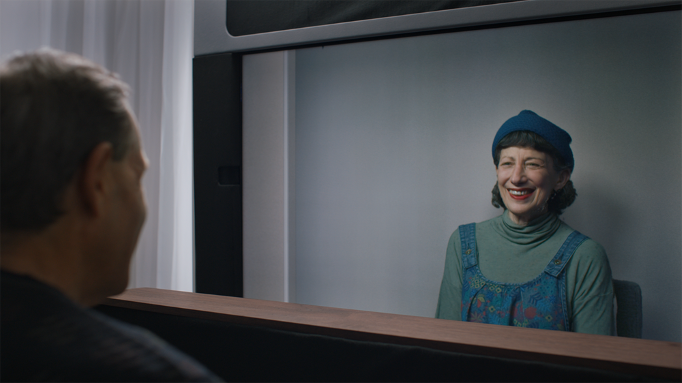
\includegraphics[width=1\columnwidth]{figures/google-starline-416.png}
    \caption{Google's Project Starline~\cite{}}
    \label{fig:google-starline}
    {\small Project Starline is reported to use a groundbreaking light field rendering system that will improve glasses-free 3D / automultiscopic video chat experience by leaps and bounds when it releases later this year.}
\end{figure}

Currently, synthesis of high-quality novel views --- the basis of Image-Based Rendering (IBR) systems --- is difficult to achieve end-to-end without some form of an intermediate representation of the structure (such as 3D world points) of the scene depicted by the given image(s). For instance, Google's Project Starline (Figure~\ref{fig:google-starline}) is reported to use a dense 3D representation to go from known views to novel views. One impressive variation of such an intermediate representation is called a Multiplane Image (MPI) --- first reintroduced in Zhou et al.~\cite{zhou2018stereo} (Figure~\ref{fig:mpi-layered-representation}). It is a volumetric representation that reprojects 2D points making up an image onto multiple 2D planes situated one behind the other at successive depths along the z-axis, according to the computed depth/disparity value(s)\footnote{Since pixels are generally smaller in size than points, there can be multiple RGBA and depth/disparity values corresponding to the multiple pixels that might make up a 2D point on an image.} at each point to be mapped. MPI planes are parallel to each other and also to a reference coordinate frame centered at a reference camera/viewpoint looking down positive z-axis. The reference camera can be that of the image itself or of a different view of the scene captured by the image. An MPI can thus be formulated as a set of RGBA layers $\{(C_1,\ \alpha_1),\ (C_2,\ \alpha_2),\ \ldots,\ (C_D,\ \alpha_D)\}$, where $C_i$ refers to the RGB map of each layer $(C_i,\ \alpha_i)$ and $\alpha_i$ is the alpha map. $D$ is the total number of depth planes used in the MPI. To render from an MPI one simply needs to alpha-blend all layers in back-to-front order, as explained in section~\ref{sec:learning-mpis}. One popular instance of such depth planes used in an MPI is a set of 32 planes positioned at equidistant disparity, with the near and far planes being at 1m and 100m in 3D world space, respectively. Since disparity is inversely proportional to depth, the points on the nearer MPI planes are closer to the reference camera than the ones on the farther planes but they have greater disparity values associated with them than the farther ones.

\begin{figure}[!h]
    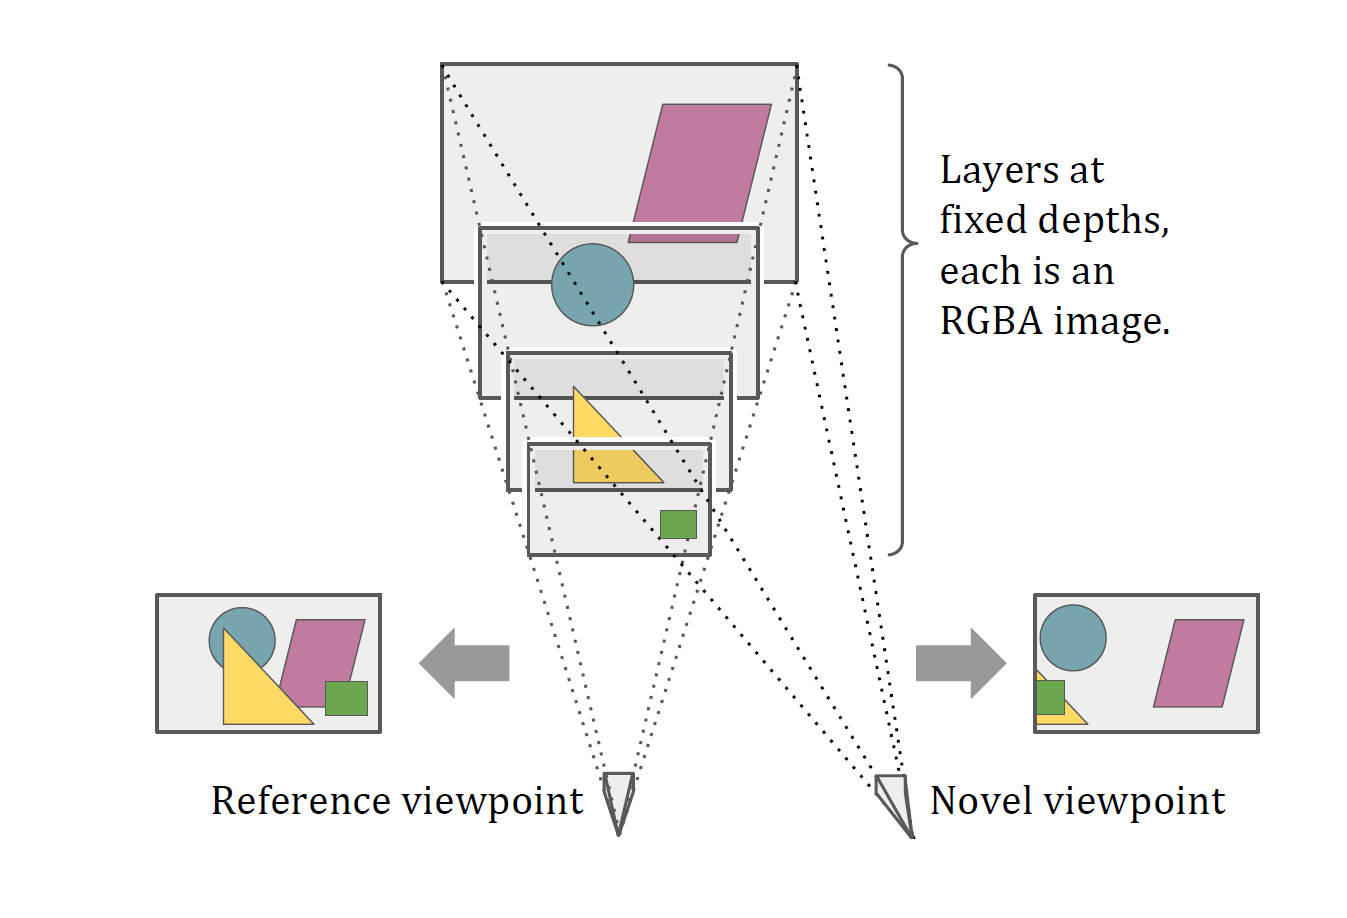
\includegraphics[width=1\columnwidth]{figures/mpi-layered-representation.png}
    \caption{The Volumetric/Layered MPI Representation}
    \label{fig:mpi-layered-representation}
    {\small A given image is reprojected onto multiple fronto-parallel MPI planes within the view frustum a common reference viewpoint that may or may not match with the given image's viewpoint. A novel image is synthesized by alpha-blending these intermediate layers in back-to-front order.}
\end{figure}

\begin{figure}[!h]
    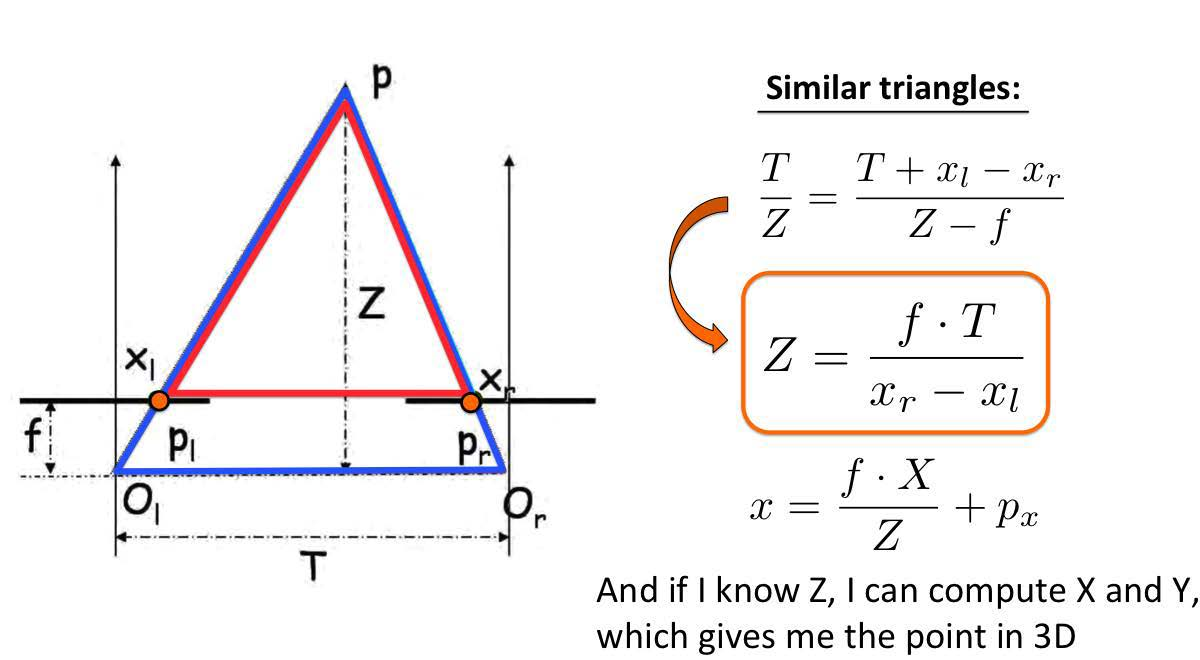
\includegraphics[width=1\columnwidth]{figures/disparity-triangulation.png}
    \caption{Disparity used in Triangulating 3D Points~\cite{fidler_depth_2021}}
    \label{fig:disparity-triangulation}
    {\small In this birds-eye view down the y-axis, $O_l$ and $O_r$ are the optical/camera centers of the left and right images of a stereo pair, $p_l$ and $p_r$ are the 2D projections of the same 3D world point $p$ onto the stereo pair, $x_l$ and $x_r$ are the x-coordinates of these 2D image points (y-coordinates are the same for corresponding points on a stereo pair), $f$ is the common focal length of the stereo cameras, $T$ is the horizontal translation or baseline of the stereo cameras, and $Z$ is the perpendicular depth of $p$ from the common reference coordinate frame of the stereo cameras and is inversely proportional to the disparity, $x_r - x_l$. Taking similar birds-eye perspectives down the $z$ and $x$ axes, we can compute the $x$ and $y$ coordinates of the 3D point as well.}
\end{figure}

Disparity refers the number of pixels that each point on a image shifts over by in any of its warped/transformed counterparts that can relate to it via a homography (projective transform function). Disparity is required for triangulating the depth(s) at each point on the image with respect to its warped version(s). Triangulating depth and estimating the 3D scene structure is easier when two or more of the scene's images are subjected to either stereo or multi-view image rectification, respectively. Such image rectification procedures typically involve rotating and shifting the optical centers of each image so they became collinear and scaling --- adjusting the focal lengths of the cameras of --- the images themselves so they become coplanar. Rectified image sets are characterized by point displacements only in the horizontal/row-wise $x$ direction. Properties of similar triangles can then be applied to the rectified images to get at the z-coordinate of each 3D world scene point most agreed upon by all the images containing the point's projections, after accounting for reprojection mismatches. Figure~\ref{fig:disparity-triangulation} shows the triangulation process for a stereo pair. This is akin to how the human visual system (including the eyes, the ganglia therein, the dorsal and ventral streams of the brain, and the visual cortex) is able to triangulate depth from binocular vision. The brain is backed by prior knowledge, heuristics, and biases (made apparent by optical illusions) that it is able to use to infer depth to some degree of approximation even with one eye closed. Since Artificial Neural Networks (ANNs) are basically trying to replicate and someday even surpass the workings of the human brain, we are actually trying to fill in for this prior knowledge acquired by the brain when we provide ANNs with copious amounts of data to learn from and devise their own heuristics out of. Therefore, we may only generate an MPI for an image when we are provided either with one or more shifted and/or rotated reprojections of the scene in the image or with the homographies for generating each of these transformed images from the original image. Otherwise, we would need to be supplied the sparse/dense 3D point cloud of the image's scene itself. 